%%%%%%%%%%%%%%%%%%%%%%%%%%%%%%%%%%%%
% Appendix A, Solution and Estimation Details
%%%%%%%%%%%%%%%%%%%%%%%%%%%%%%%%%%%%

% Set equation, figure, table indexing
\renewcommand{\thefigure}{A.\arabic{figure}}
\setcounter{figure}{0}
\renewcommand{\thetable}{A.\arabic{table}}
\setcounter{table}{0}
\renewcommand{\theequation}{A.\arabic{equation}}
\setcounter{equation}{0}
\renewcommand{\thefootnote}{A.\arabic{footnote}}
\setcounter{footnote}{0}
\section{Data} % (fold)
\label{sec:data-ap}

\begin{figure}[H]
\centering
\caption{Examples of an Implicit Association Test}
\label{fig:iatexamples}
\begin{subfigure}{.48\textwidth}
\centering
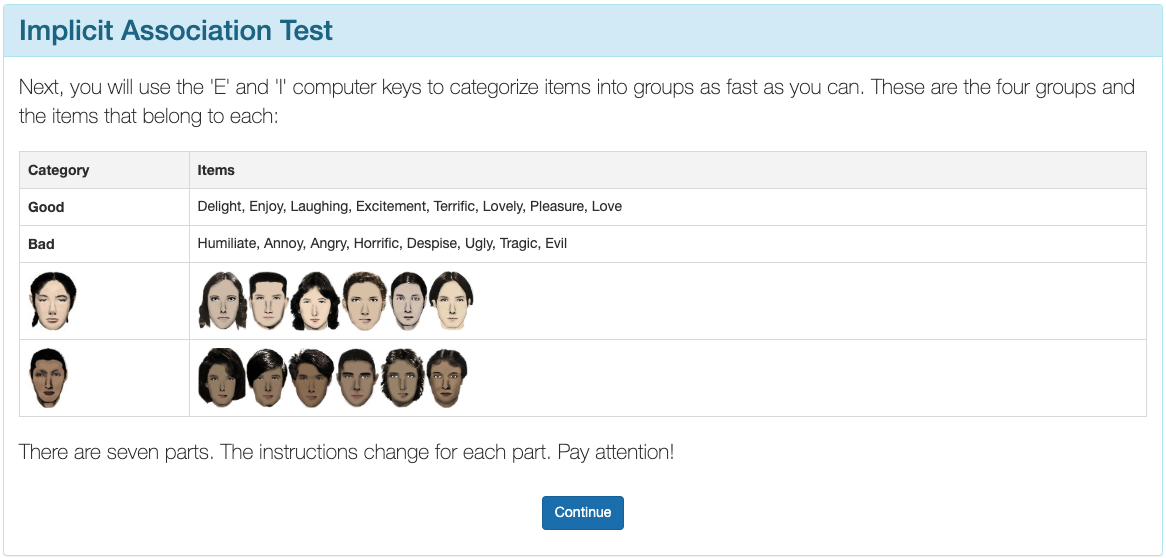
\includegraphics[width=.9\linewidth]{iatexample1.png}
\end{subfigure}
\centering
%Second graph
\begin{subfigure}{.48\textwidth}
\centering
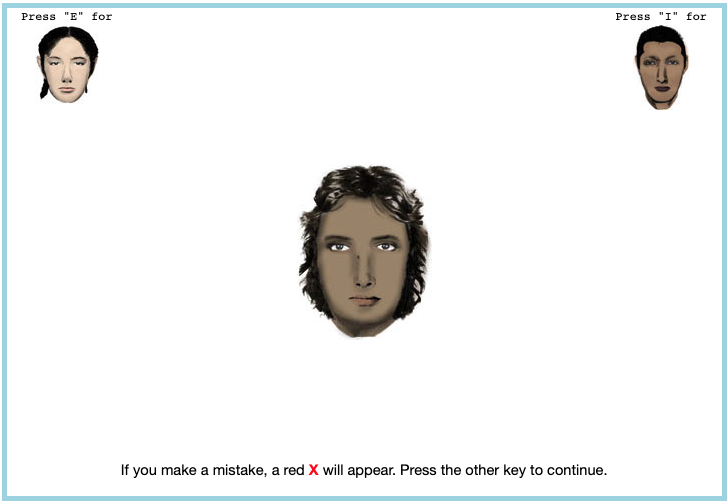
\includegraphics[width=.9\linewidth]{iatexample2.png}
\end{subfigure}
%Third
\begin{subfigure}{.48\textwidth}
\centering
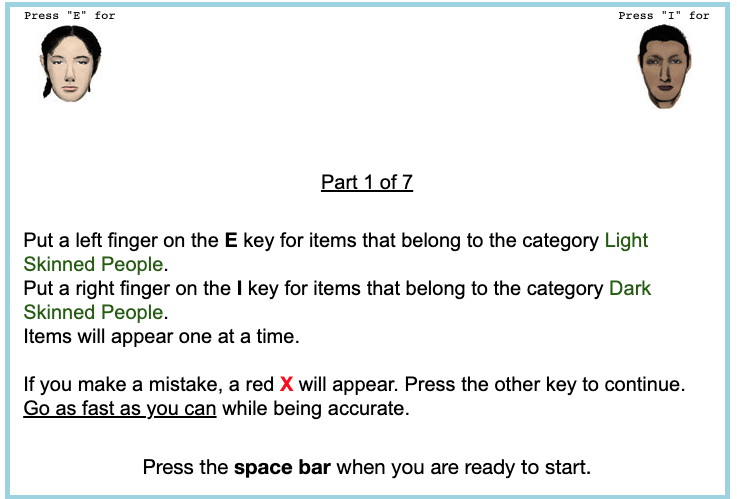
\includegraphics[width=.9\linewidth]{iatexample3.png}
\end{subfigure}
% Fourth
\begin{subfigure}{.48\textwidth}
\centering
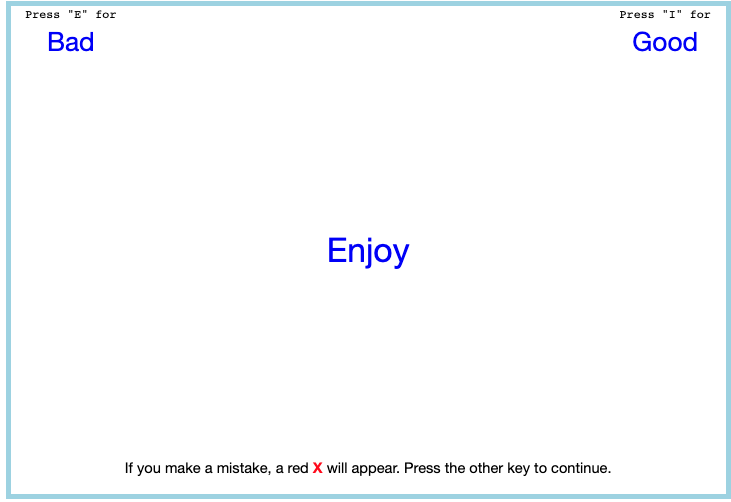
\includegraphics[width=.9\linewidth]{iatexample4.png}
\end{subfigure}
%Fifth
\begin{subfigure}{.48\textwidth}
\centering
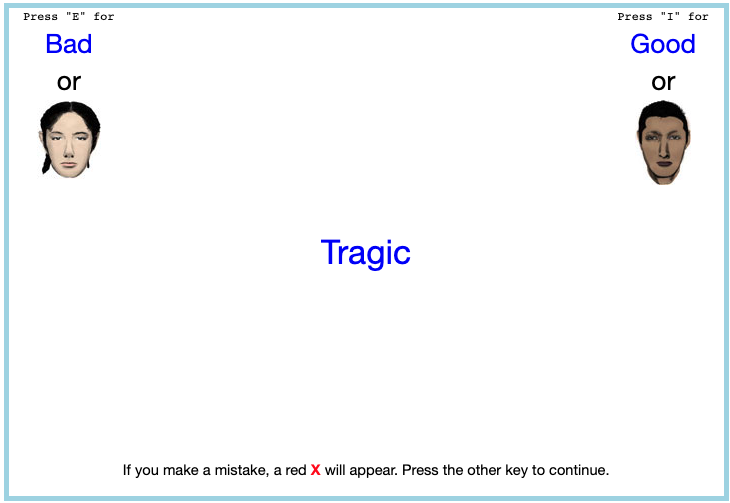
\includegraphics[width=.9\linewidth]{iatexample5.png}
\end{subfigure}
\caption*{\footnotesize{Here are a few examples of what a respondent would see on an implicit association test.}}
\end{figure}

\newpage
\pagebreak

\section{Tables} % (fold)
\label{sec:tabs-ap}

\begin{table}[!h]
\centering\centering
\caption{Subjective Asian Identity and Asian Bias \label{regtab-all-fe}}
\centering
\resizebox{\ifdim\width>\linewidth\linewidth\else\width\fi}{!}{
\begin{threeparttable}
\begin{tabular}[t]{lcccccccc}
\toprule
  & \specialcell{(1) \\ $A_i$} & \specialcell{(2) \\ $A_i$} & \specialcell{(3) \\ $A_i$} & \specialcell{(4) \\ $A_i$} & \specialcell{(5) \\ $A_i$} & \specialcell{(6) \\ $A_i$} & \specialcell{(7) \\ $A_i$} & \specialcell{(8) \\ $A_i$}\\
\midrule
Bias & $-0.04$*** & $-0.14$*** & $-0.02$*** & $-0.02$ & $-0.03$*** & $-0.07$** & $-0.10$*** & $-0.04$\\
 & ($0.01$) & ($0.04$) & ($0.01$) & ($0.03$) & ($0.01$) & ($0.03$) & ($0.03$) & ($0.03$)\\
Female & $-0.01$** & $-0.01$** & $-0.01$** & $-0.01$* & $-0.01$** & $-0.01$* & $-0.01$* & $-0.01$*\\
 & ($0.00$) & ($0.00$) & ($0.00$) & ($0.00$) & ($0.00$) & ($0.00$) & ($0.00$) & ($0.00$)\\
College Graduate: Mother & $0.01$ & $0.01$ & $0.01$ & $0.01$ & $0.01$ & $0.01$ & $0.01$ & $0.01$\\
 & ($0.01$) & ($0.01$) & ($0.01$) & ($0.01$) & ($0.01$) & ($0.01$) & ($0.01$) & \vphantom{2} ($0.01$)\\
College Graduate: Father & $0.01$** & $0.01$* & $0.01$** & $0.01$** & $0.01$** & $0.01$** & $0.01$** & $0.01$**\\
 & ($0.01$) & ($0.01$) & ($0.01$) & ($0.01$) & ($0.01$) & ($0.01$) & ($0.01$) & \vphantom{1} ($0.01$)\\
Both parents Asian & $0.63$*** & $0.63$*** & $0.62$*** & $0.62$*** & $0.63$*** & $0.63$*** & $0.63$*** & $0.62$***\\
 & ($0.03$) & ($0.03$) & ($0.03$) & ($0.03$) & ($0.03$) & ($0.03$) & ($0.03$) & ($0.03$)\\
First Gen & $0.01$ & $0.02$ & $0.02$* & $0.02$** & $0.02$* & $0.02$** & $0.02$* & $0.02$**\\
 & ($0.01$) & ($0.01$) & ($0.01$) & ($0.01$) & ($0.01$) & ($0.01$) & ($0.01$) & ($0.01$)\\
Second Gen & $0.02$ & $0.02$ & $0.01$ & $0.02$ & $0.02$ & $0.02$ & $0.02$ & $0.02$\\
 & ($0.01$) & ($0.01$) & ($0.01$) & ($0.02$) & ($0.02$) & ($0.02$) & ($0.02$) & ($0.02$)\\
\midrule
N & $129078$ & $129078$ & $129078$ & $129078$ & $129078$ & $129078$ & $129078$ & $129078$\\
Region FE &  &  &  &  & X & X &  & \\
Year FE &  & X &  & X &  & X &  & \\
State FE &  &  & X & X &  &  &  & X\\
Year-Region FE &  &  &  &  &  &  & X & X\\
\bottomrule
\multicolumn{9}{l}{\rule{0pt}{1em}* p $<$ 0.1, ** p $<$ 0.05, *** p $<$ 0.01}\\
\end{tabular}
\begin{tablenotes}
\small
\item[1] \footnotesize{I include controls for sex, quartic age, and parental education.}
\item[2] \footnotesize{Standard errors are clustered on the state level.}
\end{tablenotes}
\end{threeparttable}}
\end{table}


\newpage
\pagebreak

\begin{table}[!h]
\centering\centering
\caption{Relationship Between Bias and Self-Reported Asian Identity: By Generation \label{regtab-bygen-01}}
\centering
\resizebox{\ifdim\width>\linewidth\linewidth\else\width\fi}{!}{
\begin{threeparttable}
\begin{tabular}[t]{lcccc}
\toprule
  & \specialcell{(1) \\ All Gens \\ $H_{ist}$} & \specialcell{(2) \\  First Gen \\ $H^1_{ist}$} & \specialcell{(3) \\  Second Gen \\ $H^2_{ist}$} & \specialcell{(4) \\  Third Gen \\ $H^3_{ist}$}\\
\midrule
Bias & -0.06** & -0.05 & -0.08** & -0.08**\\
 & (0.02) & (0.04) & (0.03) & (0.03)\\
Female & 0.00 & -0.01 & 0.00 & -0.01\\
 & (0.00) & (0.01) & (0.00) & (0.01)\\
College Graduate: Mother & 0.00 & -0.01 & 0.01 & 0.03\\
 & (0.01) & (0.01) & (0.01) & \vphantom{1} (0.02)\\
College Graduate: Father & 0.00 & 0.02** & 0.00 & -0.01\\
 & (0.01) & (0.01) & (0.01) & (0.02)\\
\midrule
Observations & 129,078 & 15,499 & 80,137 & 33,442\\
Mean & 0.65 & 0.44 & 0.22 & 0.66\\
Year $\times$ Region FE & X & X & X & X\\
\bottomrule
\multicolumn{5}{l}{\rule{0pt}{1em}* p $<$ 0.1, ** p $<$ 0.05, *** p $<$ 0.01}\\
\end{tabular}
\begin{tablenotes}
\small
\item[1] \footnotesize{Each column is an estimation of a heterogeneous effect of regression (\ref{eq:identity_reg_bias}) by 
                      generation with region × year fixed effects. 
                      I include controls for sex, quartic age, fraction of Asians in a state, and parental education.
                      I also added parents' (HH, HW, and WH) and grandparents' (HHHH, HHHW, HHWH, etc.) type dummy variables to the regression
                      on second and third generation immigrants, where H is objectively Asian (born in a Asian country) and W is objectively White (native-born). 
                      Standard errors are clustered on the state level.}
\item[2] \footnotesize{The samples include children ages 17 and below who live in intact families. 
                      First-generation Asian immigrant children that were born in a 
                      Asian country. Native-born second-generation Asian 
                      immigrant children with at least one parent born in a Asian 
                      country. Finally, native-born third-generation Asian immigrant children 
                      with native-born parents and at least one grandparent born in a Asian country.}
\item[3] \footnotesize{Data source is the 2004-2021 Current Population Survey.}
\end{tablenotes}
\end{threeparttable}}
\end{table}


\newpage
\pagebreak

\begin{table}[H]

\caption{Relationship Between Bias and Self-Reported Hispanic identity Among Second-Generation Hispanic Immigrants: By Parental Type \label{regtab-byparent-01}}
\centering
\resizebox{\linewidth}{!}{
\begin{threeparttable}
\begin{tabular}[t]{lcccc}
\toprule
\multicolumn{1}{c}{Parents Type} & \multicolumn{1}{c}{All} & \multicolumn{1}{c}{\makecell[c]{Both Parents \\ from Spanish \\ Speaking Country \\ (HH)}} & \multicolumn{1}{c}{\makecell[c]{Father \\ from Spanish \\ Speaking Country \\ (HW)}} & \multicolumn{1}{c}{\makecell[c]{Mother  \\ from Spanish \\ Speaking Country \\ (WH)}} \\
\cmidrule(l{3pt}r{3pt}){1-1} \cmidrule(l{3pt}r{3pt}){2-2} \cmidrule(l{3pt}r{3pt}){3-3} \cmidrule(l{3pt}r{3pt}){4-4} \cmidrule(l{3pt}r{3pt}){5-5}
  & \specialcell{(1) \\ $H^2_{ist}$} & \specialcell{(2) \\ $H^2_{ist}$} & \specialcell{(3) \\ $H^2_{ist}$} & \specialcell{(4) \\ $H^2_{ist}$}\\
\midrule
Bias & -0.13** & -0.15** & -0.01 & -0.07\\
 & (0.05) & (0.06) & (0.07) & (0.10)\\
Female & 0.00 & 0.00 & -0.01 & 0.02**\\
 & (0.00) & (0.00) & (0.01) & (0.01)\\
College Graduate: Mother & -0.06*** & -0.04*** & -0.07*** & -0.08***\\
 & (0.01) & (0.01) & (0.01) & (0.02)\\
College Graduate: Father & -0.08*** & -0.04*** & -0.10*** & -0.11***\\
 & (0.01) & (0.01) & (0.02) & (0.01)\\
\midrule
Observations & 560,100 & 405,116 & 88,421 & 66,563\\
Year $\times$ Region FE & X & X & X & X\\
Mean & 0.94 & 0.96 & 0.9 & 0.83\\
\bottomrule
\multicolumn{5}{l}{\rule{0pt}{1em}* p $<$ 0.1, ** p $<$ 0.05, *** p $<$ 0.01}\\
\end{tabular}
\begin{tablenotes}
\small
\item[1] \footnotesize{Each column is an estimation of a heterogeneous effect of regression (\ref{eq:identity_reg_bias}) by 
                      type of parents with region × year fixed effects. 
                      I include controls for sex, quartic age, fraction of Hispanics in a state, and parental education.
                      Standard errors are clustered on the state level.}
\item[2] \footnotesize{The samples include second-generation Hispanic children ages 17 and below who live in intact families. 
                      Native-born second-generation Hispanic 
                      immigrant children with at least one parent born in a Spanish-speaking 
                      country.}
\item[3] \footnotesize{Column (1) includes the results to regression (\ref{eq:identity_reg_bias}) on all second-generation immigrants, 
                                        column (2) includes the results to regression (\ref{eq:identity_reg_bias}) on second-generation immigrants that who has a father and mother that were born in a Spanish-speaking country (HH),
                                        column (3) includes the results to regression (\ref{eq:identity_reg_bias}) on second-generation immigrants that who has a father that was born in a Spanish-speaking country and a native-born mother (HW), and
                                        column (4) includes the results to regression (\ref{eq:identity_reg_bias}) on second-generation immigrants that who has a native-born father and a mother that was born in a Spanish-speaking country (WH).}
\item[4] \footnotesize{Data source is the 2004-2021 Current Population Survey.}
\end{tablenotes}
\end{threeparttable}}
\end{table}


\newpage
\pagebreak

\begin{table}[H]
\centering\centering
\caption{Logistic Regression Analysis of Bias and Interracial Marriages \label{regtab-logit-03}}
\centering
\begin{threeparttable}
\begin{tabular}[t]{lccc}
\toprule
\multicolumn{2}{c}{ } & \multicolumn{1}{c}{Asian Men} & \multicolumn{1}{c}{Asian Women} \\
\cmidrule(l{3pt}r{3pt}){3-3} \cmidrule(l{3pt}r{3pt}){4-4}
  & \specialcell{(1) \\ Interethnic} & \specialcell{(2) \\ Interethnic} & \specialcell{(3) \\ Interethnic}\\
\midrule
Bias & $0.38$*** & $-0.19$ & $0.33$**\\
 & ($0.11$) & ($0.16$) & ($0.14$)\\
College Graduate: Wife & $0.35$*** & $0.44$*** & $0.56$***\\
 & ($0.04$) & ($0.06$) & \vphantom{1} ($0.05$)\\
College Graduate: Husband & $-0.06$ & $-0.03$ & $-0.15$***\\
 & ($0.04$) & ($0.06$) & ($0.05$)\\
\midrule
Observations & $69,800$ & $52,032$ & $60,171$\\
Year $\times$ Region FE & X & X & X\\
\bottomrule
\multicolumn{4}{l}{\rule{0pt}{1em}* p $<$ 0.1, ** p $<$ 0.05, *** p $<$ 0.01}\\
\end{tabular}
\begin{tablenotes}
\small
\item[1] \footnotesize{This is the result to estimating (\ref{eq:inter-interracial}) as a
                        logistic regression. The coefficients are exponentiated, thus should be interpreted as odds ratios.}
\item[2] \footnotesize{I include controls for partners' sex, age, education, 
                      and years since immigrating to the United States.
                      Standard errors are clustered on the household level.}
\item[3] \footnotesize{Data source is the 2004-2020 Current Population Survey Data.}
\end{tablenotes}
\end{threeparttable}
\end{table}


\newpage
\pagebreak

\section{Figures}\label{appendix:figs}

\begin{figure}[H]
    \centering
    \caption{Scatter Plot of Proportion Subjectively Asian on Bias}
    \label{scatter-plot-1}
    \begin{subfigure}{.9\textwidth}
    \caption{Year < 2015}
    \centering
    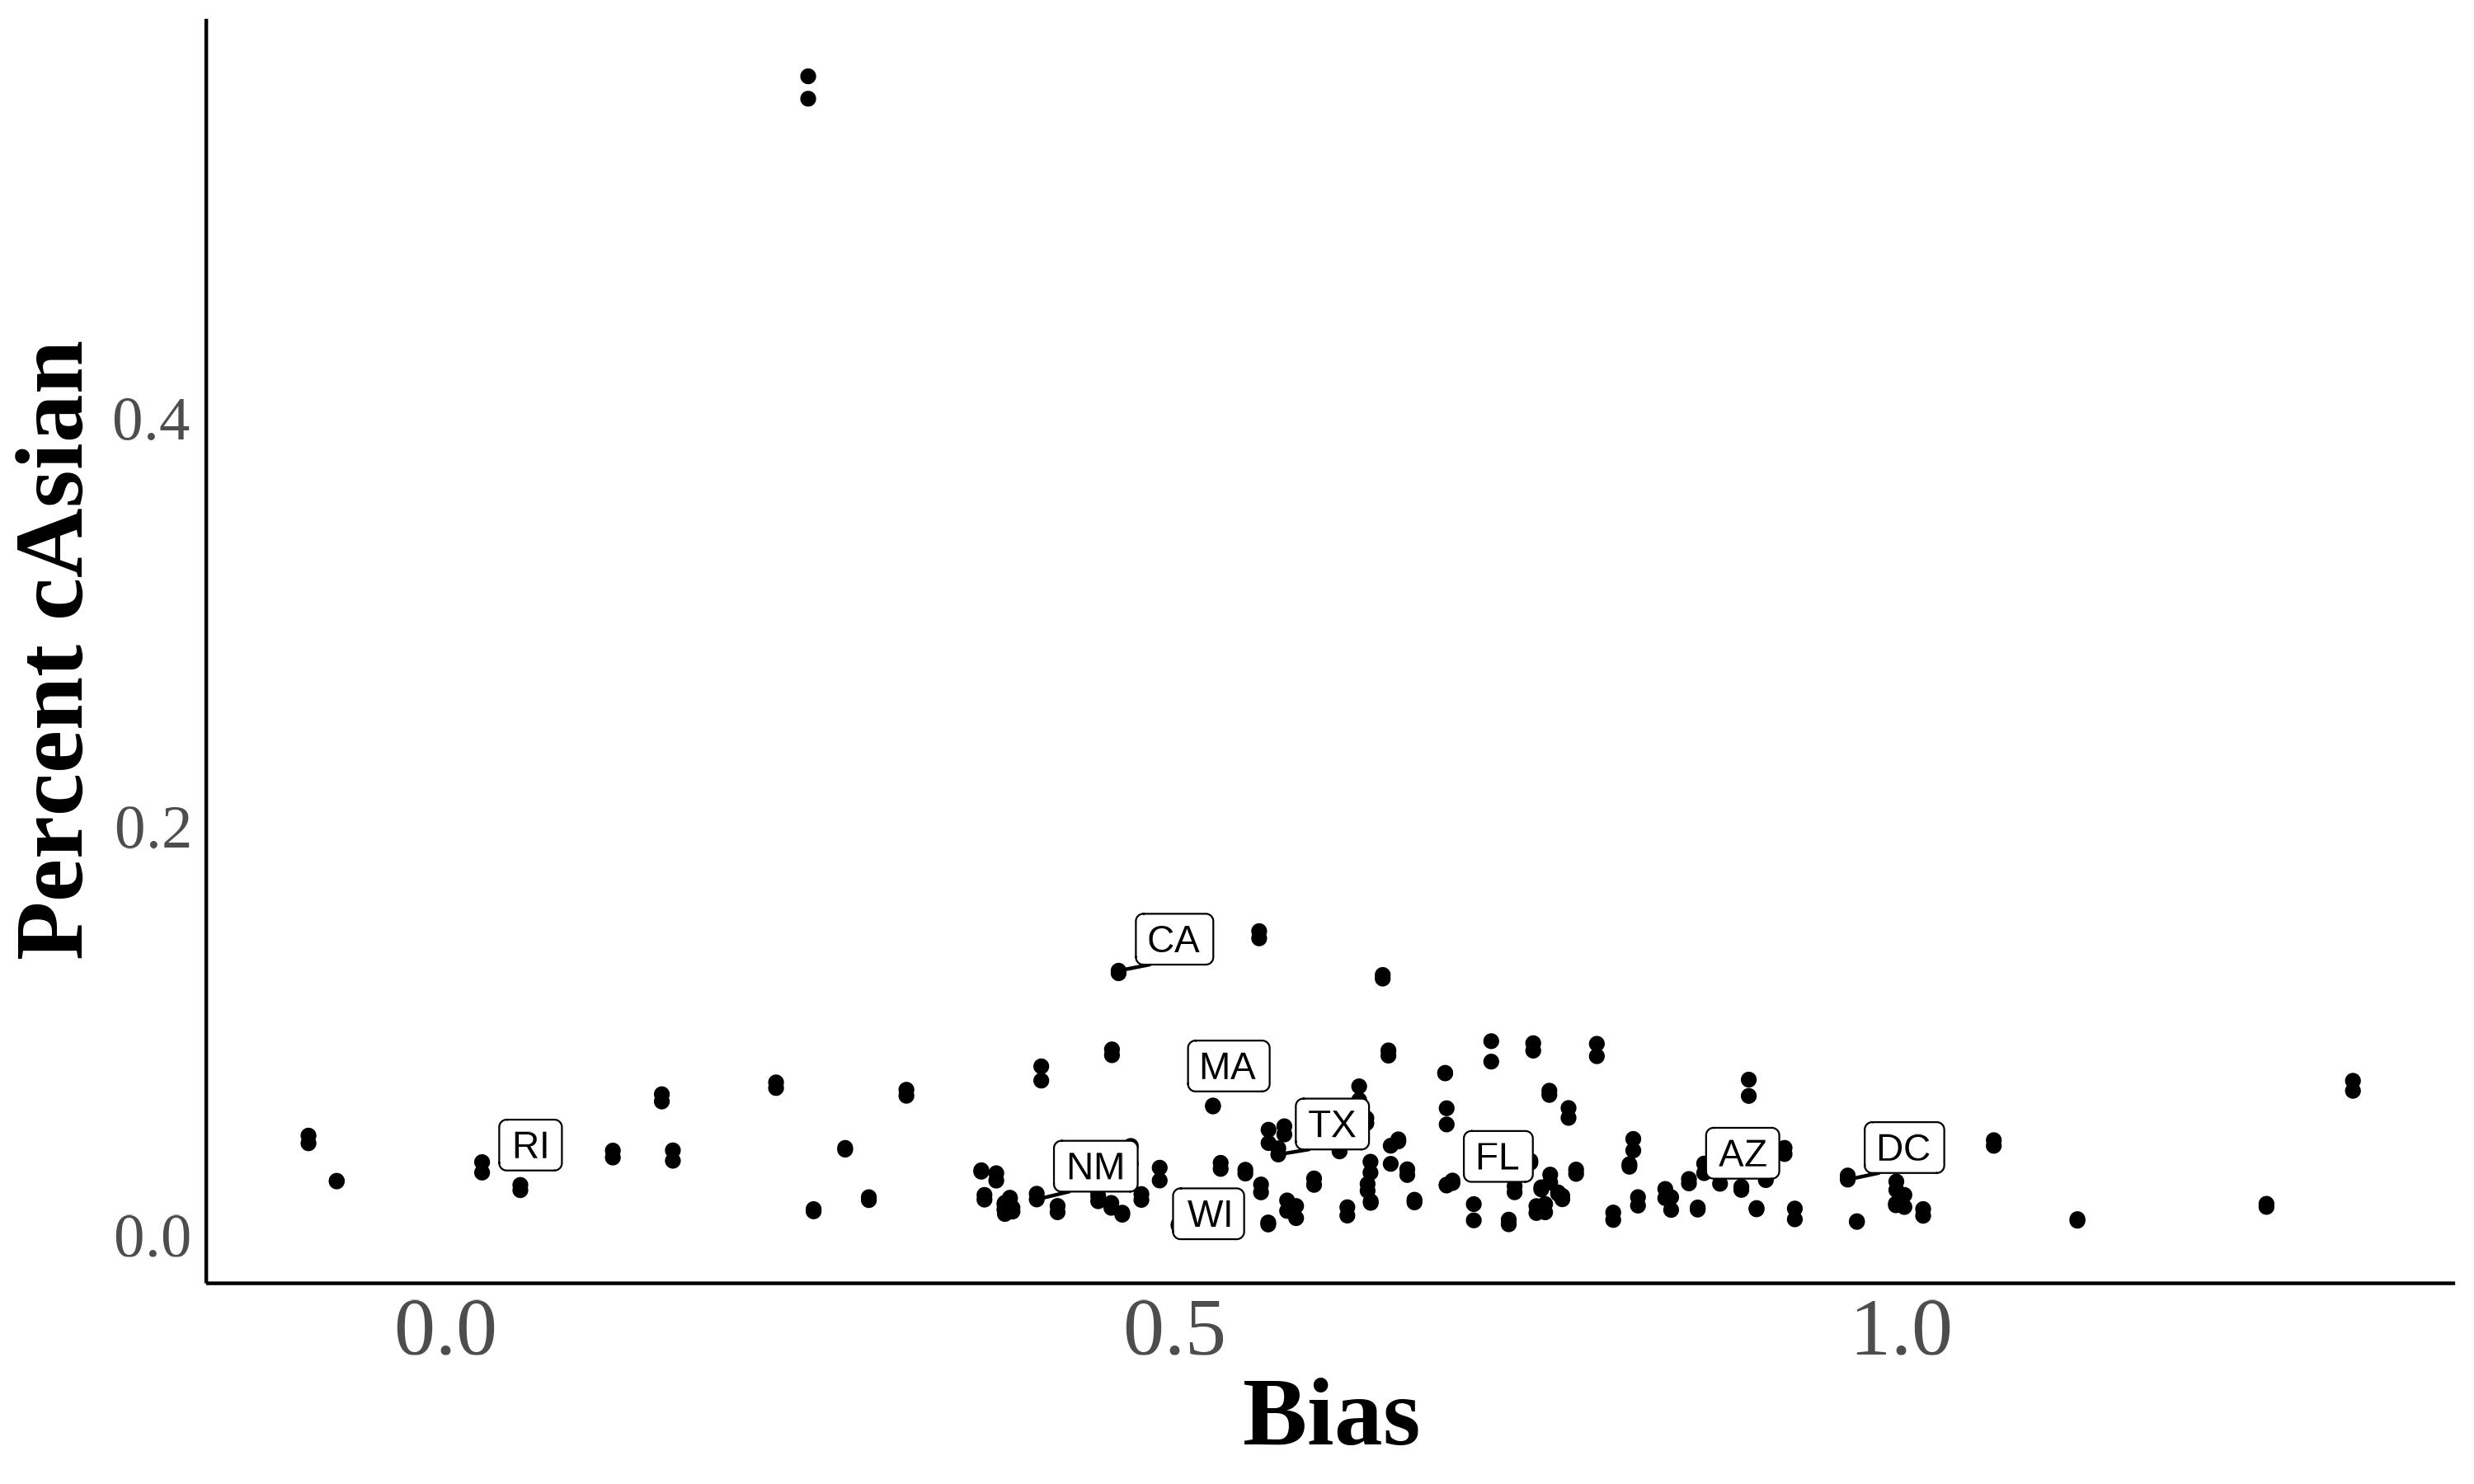
\includegraphics[width=.9\linewidth]{scatter-plot-bias-Asian-less2015.png}
    \end{subfigure}
    \centering
    %Second graph
    \begin{subfigure}{.9\textwidth}
    \caption{Year $\geq$ 2015}
    \centering
    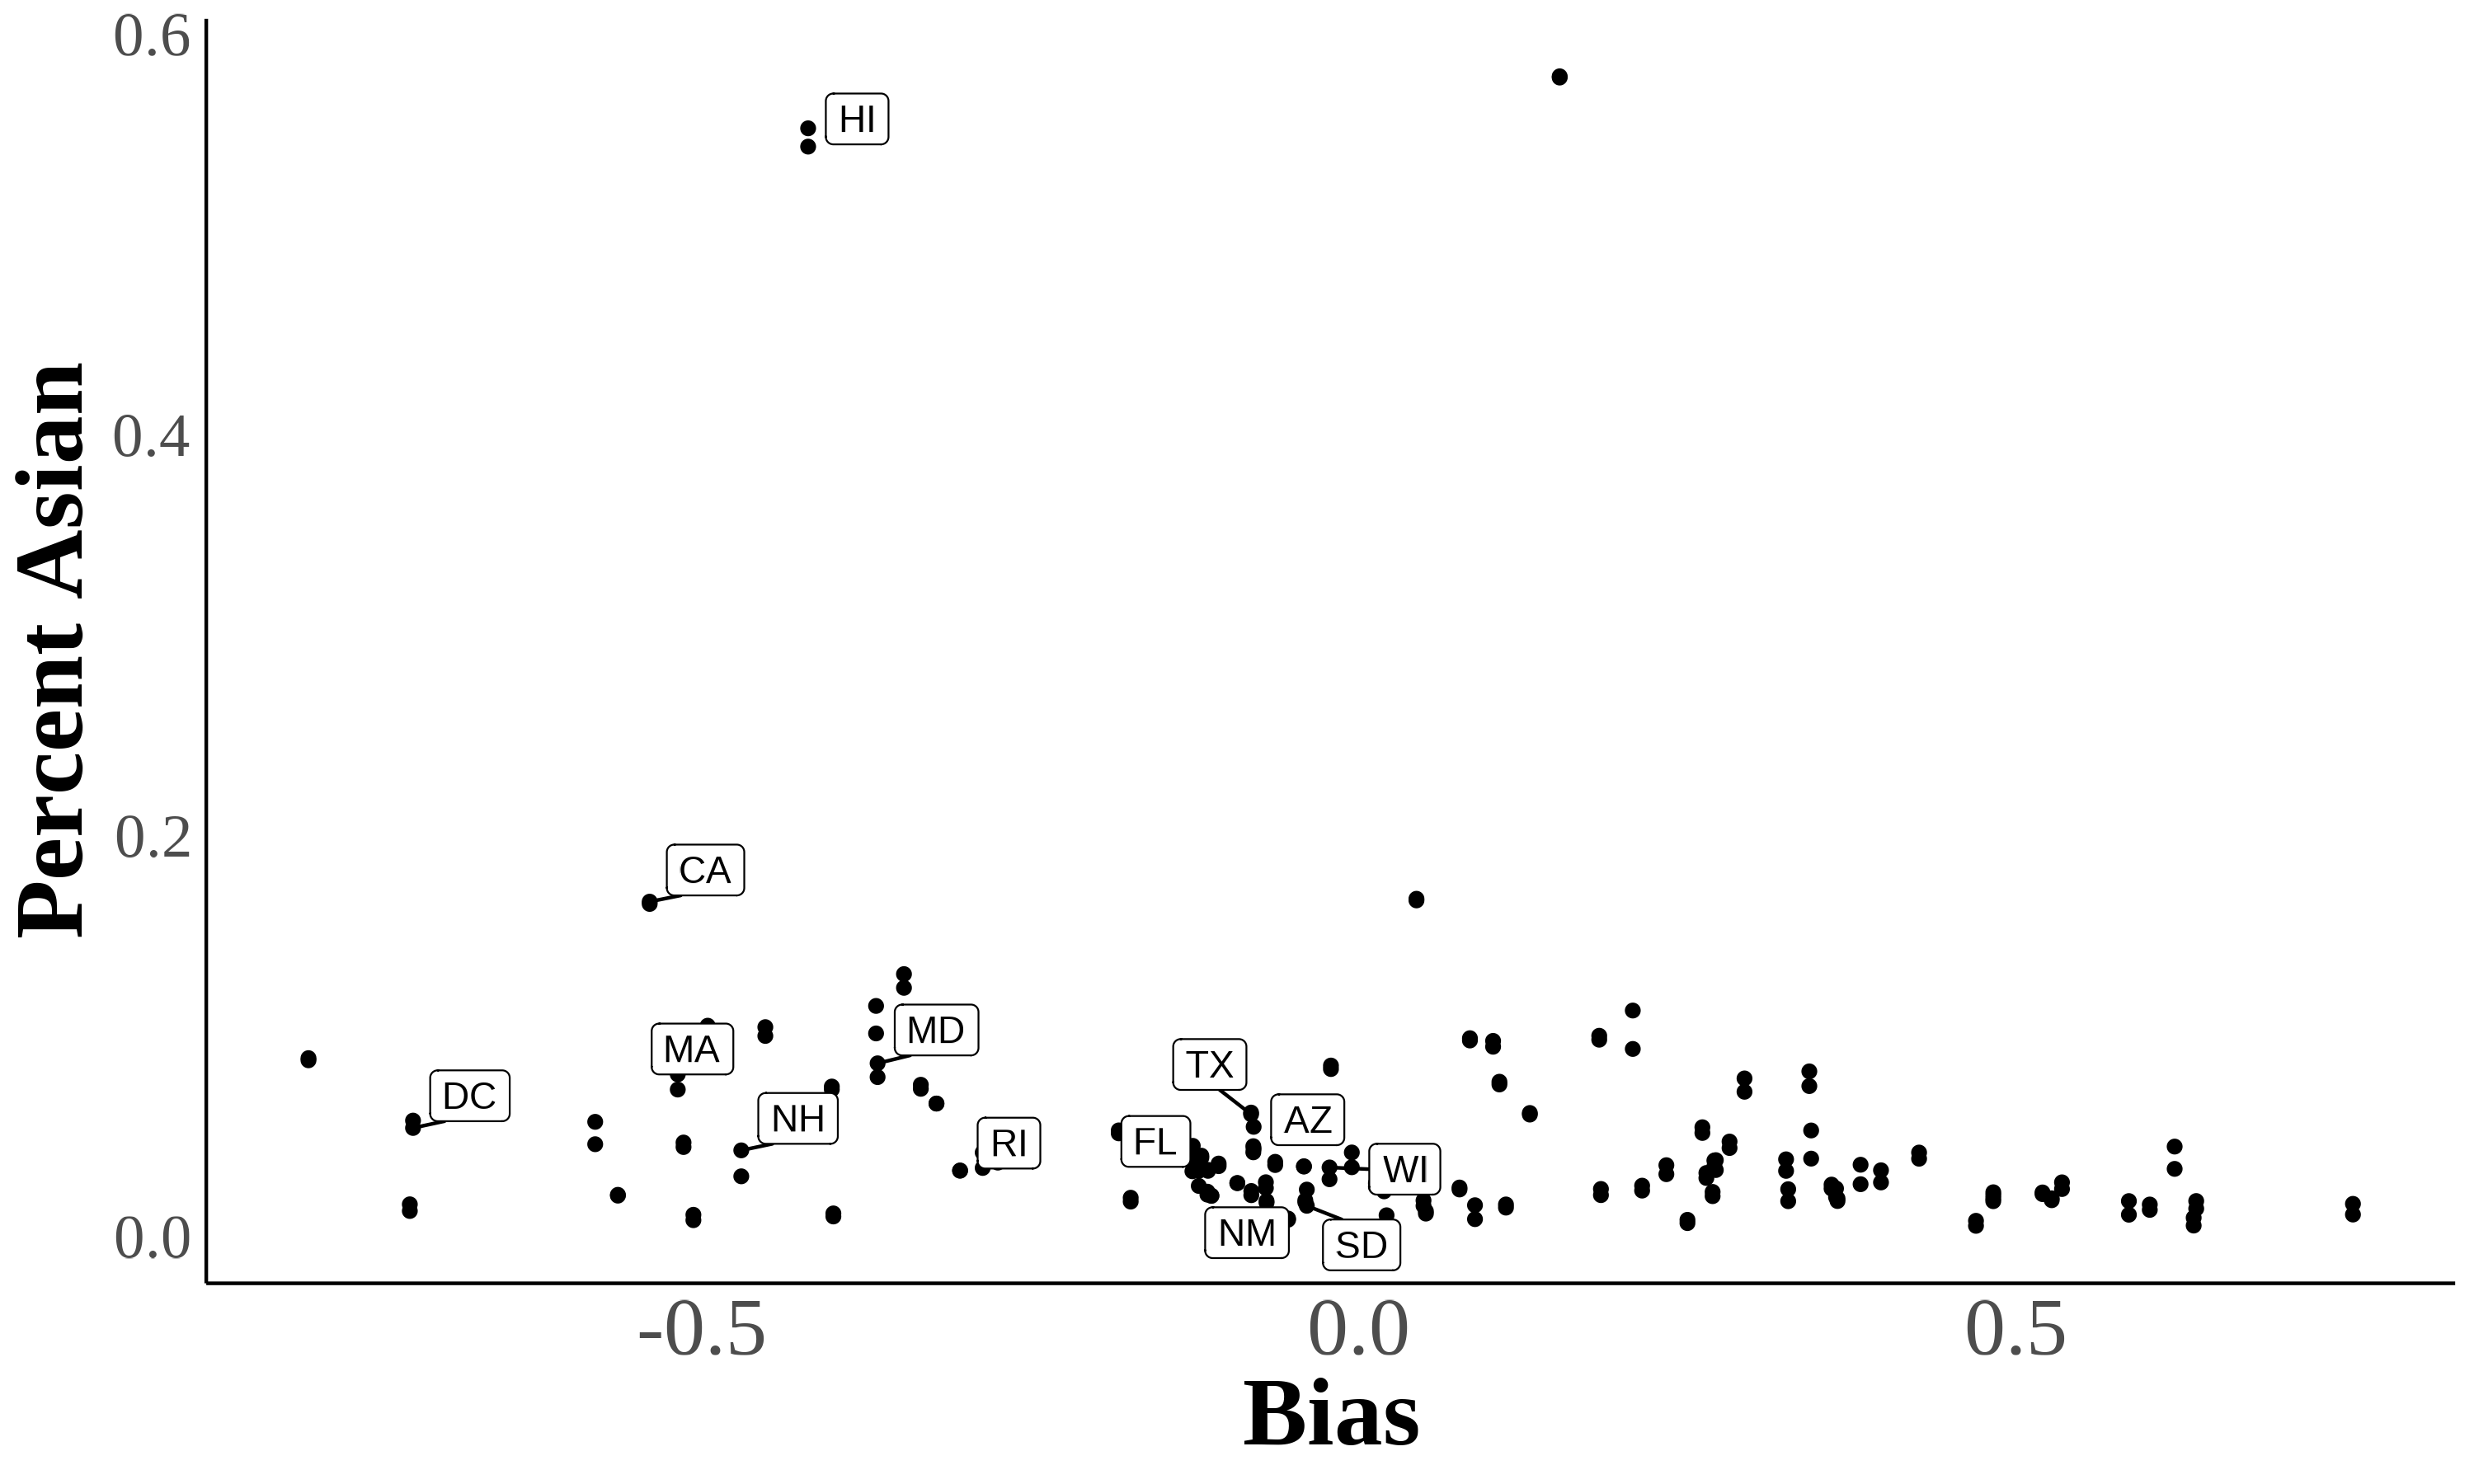
\includegraphics[width=.9\linewidth]{scatter-plot-bias-Asian-great2015.png}
    \end{subfigure}
    \caption*{\footnotesize{Here are two scatter plots showing the relationship between bias and subjective Asian population in a state. Each dot represents a state in a certain year. Percent subjectively Asian = $\frac{\# \text{Asian}}{\text{Population}}$ \\
    \emph{Source.} 2004-2021 Current Population Survey.}}
    \end{figure}
    
\subsection{Using \textcite{lubotskyInterpretationRegressionsMultiple2006} to Construct Bias Index} % (fold)
\label{sub:lw-bias}
In \textcite{lubotskyInterpretationRegressionsMultiple2006}, the authors propose a method to reduce measurement error in proxies by constructing a composite index. The Lubotsky-Wittenberg (henceforth LW) consider a model where a covariate is unobserved. Therefore, they use two proxies in its place, which will have measurement error. Thus, the LW method allows researchers to use two proxies that are error-ridden. 

LW consider a setup with the following model:

\begin{align*}
    y &= \alpha + \beta x^* + \epsilon \\
    x_1 &= x^* + \mu_1 \\
    x_2 &= x^* + \mu_2
\end{align*}

Where \(x_{i}^{*}\) is the unobserved covariate, \(x_{1i}\) and \(x_{2i}\) are the proxies, and the measurement errors \(\mu_1\) and \(\mu_2\) are assumed to be classical and allowed to covary. The covariance matrix of the errors is given by:

\[
\Sigma = \begin{bmatrix}
    \sigma_1^2 & \sigma_{12} \\
    \sigma_{12} & \sigma_2^2
\end{bmatrix}
\]

Replacing the unobserved \(x^*\) with \(x_1\) or \(x_2\) yields the following expectations of the OLS estimates:

\[
\mathbb{E} \left[ \hat{\beta}_1 \right] = \beta \frac{\sigma_{x^*}^2}{\sigma_{x^*}^2 + \sigma_1^2} \quad ; \quad \mathbb{E} \left[ \hat{\beta}_2 \right] = \beta \frac{\sigma_{x^*}^2}{\sigma_{x^*}^2 + \sigma_2^2}
\]

Both estimates are biased; the one with the smaller variance of the measurement error being less biased.

LW then propose defining a new proxy \(x_3\) as a weighted average of \(x_1\) and \(x_2\):

\[
x_3 = \lambda x_1 + (1 - \lambda) x_2
\]

To minimize the attenuation bias in the OLS estimate of \(\beta\), they solve for the optimal value of \(\lambda\):

\[
\lambda^* = \frac{\sigma_2^2 - \sigma_{12}}{\sigma_1^2 + \sigma_2^2 - 2\sigma_{12}}
\]

This optimal value of \(\lambda\) is not directly useful because the variances of the measurement errors and their covariance are unobserved. However, if you estimate a bivariate regression using OLS (i.e., regress \(y\) on \(x_1\) and \(x_2\)), then the expectation of the sum of the two coefficient estimates is identical to the expectation of the OLS coefficient estimate on \(x_3\) in a univariate regression using the optimal choice of \(\lambda\):

\[
\mathbb{E} \left[ \hat{\beta}_1 + \hat{\beta}_2 \right] = \mathbb{E} \left[ \hat{\beta}_{x_3} \right]
\]

Thus, OLS produces an estimate of \(\beta\) with the least bias by optimally combining the information in \(x_1\) and \(x_2\).
